\chapter{Data science project}

\chapterprecishere{Figured I could throw myself a pity party or go back to school and
learn the computers. \par\raggedleft--- \textup{Don Carlton}, Monsters University (2013)}

First of all, a data science project is a software project.  The difference between a data
science software and a traditional software is that some components of the former is
constructed from data.  This means that part of the solution cannot be designed from the
knowledge of the domain expert, but must be learned from the data.  (Alternatively, the
cost of designing the solution is too high, and it is more efficient to learn it from the data.)

One good example of a data science project is a spam filter.  The spam filter is a software
that classifies emails into two categories: spam and non-spam.  The software is trained
using a set of emails that are already classified as spam or non-spam.  The software is
then used to classify new emails.  The software is a data science software because the
classification algorithm is learned from the data, i.e. the filters are not designed ``by
hand''.

% TODO:
% - the need of methodologies for data science projects
% - CRISP-DM
% - Nina's approach
% - Agile
% - Problems and advantages of SCRUM
% - Our approach

\section{CRISP-DM}

CRISP-DM\footnote{Official guide available at
\url{https://www.ibm.com/docs/it/SS3RA7_18.3.0/pdf/ModelerCRISPDM.pdf}.} is a methodology
for data mining projects.  It is an acronym for Cross Industry Standard Process for Data
Mining.  It is a methodology that was developed in the 1990s by IBM, and it is still
widely used today.

CRISP-DM is a cyclic process.  The process is composed of six phases:
\begin{enumerate}
  \item Business understanding: this is the phase where the project objectives are
    defined.  The objectives must be defined in a way that is measurable.  The phase also
    includes the definition of the project plan.
  \item Data understanding: this is the phase where the data is collected and explored.
    The data is collected from the data sources, and it is explored to understand its
    characteristics.  The phase also includes the definition of the data quality
    requirements.
  \item Data preparation: this is the phase where the data is prepared for the modeling
    phase.  The data is cleaned, transformed, and aggregated.  The phase also includes the
    definition of the modeling requirements.
  \item Modeling: this is the phase where the model is trained and validated.  The model is
    trained using the prepared data, and it is validated using the validation data.  The
    phase also includes the definition of the evaluation requirements.
  \item Evaluation: this is the phase where the model is evaluated.  The model is evaluated
    using the evaluation data.  The phase also includes the definition of the deployment
    requirements.
  \item Deployment: this is the phase where the model is deployed.  The model is deployed
    using the deployment requirements.  The phase also includes the definition of the
    monitoring requirements.
\end{enumerate}

\Cref{fig:cripdm} shows a diagram of the CRISP-DM process.  Note that the process is
cyclic and completly focused on the data.  The process do not address the software
development aspects of the project.


\tikzset{%
  block/.style={rectangle, draw, text width=6em, text centered, rounded corners, minimum height=3em},
  line/.style={draw, -latex},
  dline/.style={draw, latex-latex},
  bigarrow/.style={draw, -latex, line width=3pt, gray}}

\begin{figurebox}[label=fig:cripdm]{Diagram of the CRISP-DM process.}
  \centering
  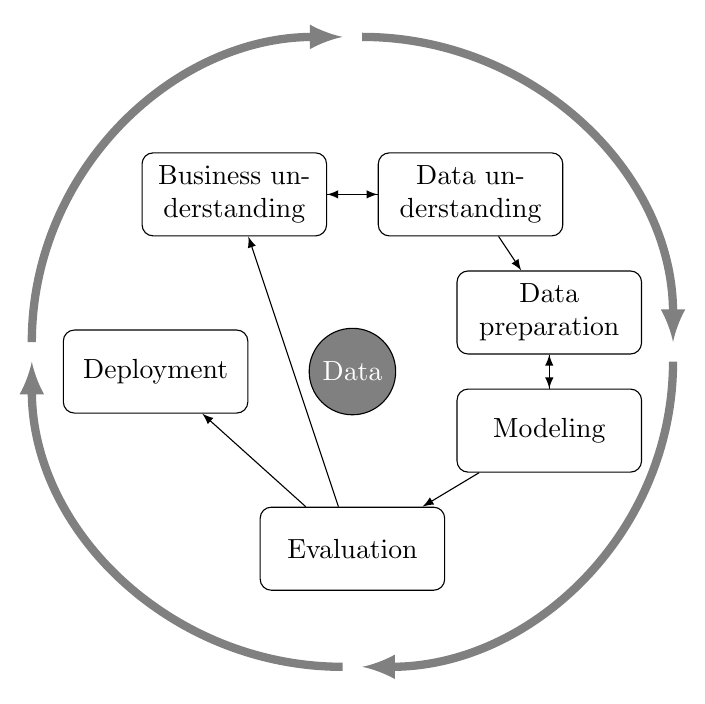
\begin{tikzpicture}
    \node (1) at (0, 0) {};
    \node (2) at (4, -4) {};
    \node (3) at (0, -8) {};
    \node (4) at (-4, -4) {};

    \node [block] (bu) at (-1.5, -2) {Business understanding};
    \node [block] (du) at (1.5, -2) {Data understanding};
    \path [line] (bu) -- (du);
    \path [line] (du) -- (bu);

    \node [block] (dp) at (2.5, -3.5) {Data preparation};
    \node [block] (m) at (2.5, -5) {Modeling};
    \path [line] (dp) -- (m);
    \path [line] (m) -- (dp);

    \path [line] (du) -- (dp);

    \node [block] (e) at (0, -6.5) {Evaluation};
    \node [block] (d) at (-2.5, -4.25) {Deployment};

    \path [line] (m) -- (e);
    \path [line] (e) -- (d);
    \path [line] (e) -- (bu);

    \node [draw, circle, fill=gray, text centered, text=white] at (0, -4.25) {Data};

    \path [bigarrow] (1.east) to[out=0, in=90] (2.60);
    \path [bigarrow] (2.-60) to[out=-90, in=0] (3.east);
    \path [bigarrow] (3.west) to[out=180, in=-90] (4.-120);
    \path [bigarrow] (4.120) to[out=90, in=180] (1.west);
  \end{tikzpicture}
  \tcblower
  Each block represents a phase of the CRISP-DM process.  Data is the central element of
  the process.  Arrows represent the transitions between the phases.
\end{figurebox}

The CRISP-DM methodology is a good starting point for data science projects.  However, it
does not mean that should be followed strictly.  The process is cyclic and flexible, and
adaptations are possible at any stage of the process.

\section{Nina and Zumel's approach}

\textcite{Zumel2019} also propose a methodology for data science projects.  Besides
describing each step in a data science project, they further address the roles of each
individual involved in the project.  They state that data science projects are always
collaborative, as they require domain expertise, data expertise, and software expertise.
The requirements are dynamic, and the project has many exploratory phases.  Usually,
projects based on data are urgent, and they must be completed in a short time --- not
only due to the business requirements, but also because the data changes over time.
The authors state that agile methodologies are suitable (and necessary) for data science
projects.

\subsection{Roles}

In their approach, five roles are defined.

\paragraph{Project sponsor}  It is the main stakeholder of the project, the one that needs the
results of the project.  He represents the business interests and champions the project.
The project is considered successful if the sponsor is satisfied.  Note that, ideally, the
sponsor can not be the data scientist, but someone that is not involved in the development
of the project.  However, he needs to be able to express \emph{quantitatively} the business
goals and participate actively in the project.

\paragraph{Client}  The client is the domain expert.  He represents the end users'
interests.  In a small project, he is usually the sponsor.  He translates the daily
activities of the business into the technical requirements of the software.

\paragraph{Data scientist}  The data scientist is the one that sets and executes the
analytic strategy.  He is the one that communicates with the sponsor and the client,
effectively connecting all the roles.  In small projects, he can also act as the developer
of the software.  However, in large projects, he is usually the project manager.
Although it is not required to be a domain expert, the data scientist must be able to
understand the domain of the problem.  He must be able to understand the business goals and
the client's requirements.  Most importantly, he must be able to define and to solve the
right tasks.

\paragraph{Data architect}  The data architect is the one that manages data and data storage.
He usually is involved in more than one project, so it is not an active participant.  He
that receives instructions to adapt the data storage and means to collect data.

\paragraph{Operations}  The operations role is the one that manages infrastructure and
deploys final project results.  He is responsible to define requirements such as response
time, programming language, and the infrastructure to run the software.

\subsection{Process}

\citeauthor{Zumel2019}'s model is similar to CRISP-DM, but emphasizes that back-and-forth
is possible at any stage of the process.  \Cref{fig:zumel} shows a diagram of the process.
The phases are:
\begin{itemize}
  \item Define the goal: what problem are we trying to solve?
  \item Collect and manage data: what information do we need?
  \item Build the model: find patterns in the data that may solve the problem.
  \item Evaluate the model: is the model good enough to solve the problem?
  \item Present results and document: establish that we can solve the problem and how we
    did it.
  \item Deploy the model: make the model available to the end users.
\end{itemize}

\begin{figurebox}[label=fig:zumel]{Diagram of the data science process proposed by \textcite{Zumel2019}.}
  \centering
  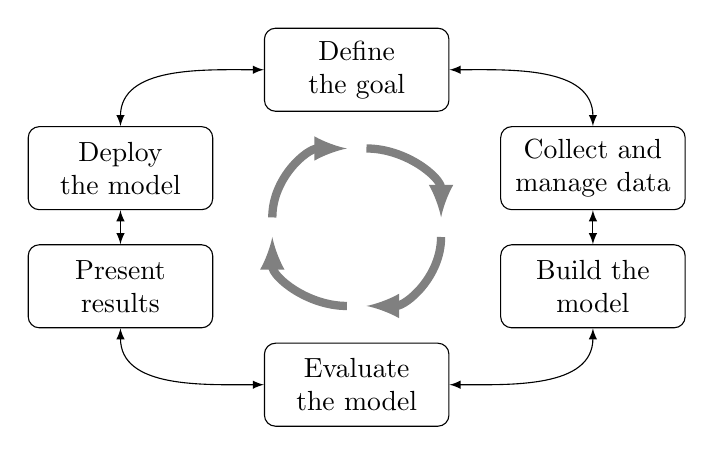
\begin{tikzpicture}
    \node (1) at (0, 0) {};
    \node (2) at (1, -1) {};
    \node (3) at (0, -2) {};
    \node (4) at (-1, -1) {};
    \path [bigarrow] (1.east) to[out=0, in=90] (2.60);
    \path [bigarrow] (2.-60) to[out=-90, in=0] (3.east);
    \path [bigarrow] (3.west) to[out=180, in=-90] (4.-120);
    \path [bigarrow] (4.120) to[out=90, in=180] (1.west);

    \node [block] (dg) at (0, 1) {Define the goal};
    \node [block] (cm) at (3, -0.25) {Collect and manage data};
    \node [block] (bm) at (3, -1.75) {Build the model};
    \node [block] (em) at (0, -3) {Evaluate the model};
    \node [block] (pd) at (-3, -1.75) {Present results};
    \node [block] (dm) at (-3, -0.25) {Deploy the model};

    \path [dline] (dg) to[out=0, in=90] (cm.north);
    \path [dline] (cm) -- (bm);
    \path [dline] (bm.south) to[out=-90, in=0] (em.east);
    \path [dline] (em.west) to[out=180, in=-90] (pd.south);
    \path [dline] (pd) -- (dm);
    \path [dline] (dm.north) to[in=180, out=90] (dg.west);
  \end{tikzpicture}

  \tcblower
  Each block represents a phase of the data science process.  The emphasis is on the
  cyclic nature of the process.  Arrows represent the transitions between the phases, that
  can be back-and-forth.
\end{figurebox}

\section{Agile}

Agile is a methodology for software development.  It is an alternative to the waterfall
methodology.  The waterfall methodology is a sequential design where each phase
must be completed before the next phase can begin.

The four values of agile manifesto are:
\begin{itemize}
  \item Individuals and interactions over processes and tools;
  \item Working software over comprehensive documentation;
  \item Customer collaboration over contract negotiation;
  \item Responding to change over following a plan.
\end{itemize}

\section{SCRUM}

SCRUM is an agile framework for software development.  It is a process framework for
managing complex projects.  It is a lightweight, which means that it
provides just enough guidance to be effective.

Many consider that SCRUM is not adequate for data science projects.  The main reason is
that SCRUM is designed for projects where the requirements are known in advance.  Also,
that data science projects have exploratory phases, which are not well supported by SCRUM.

I argue that this view is wrong.  SCRUM is a framework, and it is designed to be adapted to
the needs of the project.  SCRUM is not a rigid process.  In the following, I propose an
extension to SCRUM that makes it suitable for data science projects.

(In real-world, most developers do not have hacking-level skills.  They are not autonomous
enough to work without a plan.  This is especially true for ``data scientists,'' who are
often not even developers.  SCRUM is a good compromise between the need for autonomy and
the need for a detailed plan.  Project methodology is needed to ensure that the project is
completed in time and within budget.)

\section{Our approach}

The previously mentioned methodologies lack the focus on the software development aspects of
the data science project.  For instance, CRISP-DM defines the stages only of the data
mining process, i.e. it does not explicitly address user interface or data collection.
\citeauthor{Zumel2019}'s approach addresses data collection and presentation of results, but
delegates the software development to the operations role, barely mentioning it.  SCRUM is
a good framework for software development, but it is not designed for data science
projects.  It lacks the exploratory phases of data science projects.

Thus, we propose an extension to SCRUM that makes it suitable for data science projects.
The extension is based on the following observations:
\begin{itemize}
  \item Data science projects have exploratory phases;
  \item Data itself is a component of the solution;
  \item The solution is usually modularized, parts of it are constructed from data while the
    other parts are constructed like traditional software;
  \item The solution is usually deployed as a service, that must be maintained and
    monitored.
\end{itemize}

Moreover, we add two other values besides the agile manifesto values.  They are:
\begin{itemize}
  \item Model confidence/understanding over model performance;
  \item Code version control over interactive environments.
\end{itemize}

The first value is based on the observation that the model performance is not the most
important aspect of the model.  The most important aspect is the being sure that the model
behaves as expected (and sometimes why it behaves as expected).  It is not uncommon to find
models that seems to perform well during evaluation steps\footnote{Of course, when
evaluation is not performed correctly.}, but that are not suitable for production.

The second value is based on the observation that interactive environments are not suitable
for the development of the model search code, for instance.  Interactive environments
auxiliate the exploratory phases, but the final version of the code must be version
controlled.  Often, we hear stories that models cannot be reproduced because the code that
generated them are not runnable anymore.  This is a serious problem, and it is not
acceptable for maintaining a software solution.

These observations and values are the basis of our approach.  The roles and principles of
our approach are described in the following sections.

\subsection{The roles of our approach}

\textcolor{red}{Combine SCRUM roles with the roles defined by \textcite{Zumel2019}.}

\subsection{The principles of our approach}

\begin{enumerate}
  \item Modularize the solution. Usually, in four main modules: frontend, backend,
    dataset, and model search.  The frontend is the user interface.  The backend is the
    server-side code.  The dataset is the data that is used to train the model.  The model
    search is the code that searches for the best model.
  \item Version control everything.  This includes the code, the data, and the
    documentation. The most used tool for code version control is Git.  For datasets,
    extensions to Git exist, such as DVC\footnote{\url{https://dvc.org/}}.  One important aspect
    is to version control the model search code.  Interactive environments such as Jupyter
    notebooks are not suitable for this purpose.  They can be used to draft the code, but
    the final version must be version controlled.
  \item Continuous integration and continuous deployment.  This means that the code is
    automatically (or at least semi-automatically) tested and deployed.  The backend and
    frontend code is tested using unit tests.  The model search code is tested using
    validation methods such as cross-validation and Bayesian analysis on the discovered
    models.  Usually the model search code is very computationally intensive, and it is
    not feasible to run it on every commit.  Instead, it is run periodically, for example
    once a day.  If the clould infrastructure required to run the model search code is not
    available to automate validation and deploymen, at least make sure that the code is
    easily runnable.  This means that the code must be well documented, and that the
    required infrastructure must be well documented.  Also aggregate commands using a
    Makefile or a similar tool.  Pay attention on the dependences between dataset and the
    model training.  If the dataset changes significantly, not only the deployed model
    must be retrained, but the model search algorithm may need to be rethought.
  \item Reports as deliverables.  During sprints, the deliverables of data exploration are
    reports.  The reports must be version controlled and must be reproducible.  The reports
    must be generated in a way that is understandable by the client and the sponsor.
  \item Setup quantitative goals.  Do not fall on the trap of forever improving the model.
    Instead, setup quantitative goals for the model performance.  For example, the model
    must have a precision of at least 90\%.  Once you reach the goal, prioritize other
    tasks.
  \item Measure \emph{exactly} what you want.  During model validation, use your own
    metrics based on the project goals.  Usually, more than one metric is needed, and they
    might be conflicting.  Use strategies to balance the metrics, such as Pareto
    optimization.  Beware of the metrics that are most used in the literature.  They might not
    be suitable for your project.  Notice that during model training, some methods are
    limited to the loss functions that they can optimize.  If possible, choose a method
    that can optimize the loss function that you want.  Even if you are not explicitly
    optimizing the wanted metric, you might find a model that performs well on that metric.
    That is a reason validation is important.
  \item Report model stability and performance variance.  Understanding the limitations
    and characteristics of the model is more important than the model performance.  For
    example, if the model performance is high, but the model is unstable, it is not
    suitable for production.  Also, in some scenarios, interpretability is more important than
    performance.
  \item In user interface, mask data-science-specific terminology.  Usually, data science
    software gives the user the option to choose the model.  In order to avoid confusion,
    the user interface must mask the data-science-specific terminology.  This helps non
    experts to use the software consciously.
  \item Monitor model performance in production.  If possible setup feedback from the user
    interface.  Avoid automation of model releases because concept drift usually requires
    exploratory analysis.
  \item Use the appropriate backend.  REST API vs websocket.  The choice depends on the
    requirements of the project.  REST API is more suitable for stateless requests, while
    websocket is more suitable for stateful requests.  For example, if the user interface
    must be updated in real-time, websocket is more suitable.  If the user interface is
    used to submit batch requests, REST API is more suitable.
\end{enumerate}
